\documentclass[twoside,onecolumn,10pt]{waflarticle}
% can use option mtpro 

\usepackage{graphicx}
\usepackage{rotating}
\usepackage{scalefnt}
\usepackage{bm}
\usepackage{fancyhdr}
\usepackage{etoolbox}
\usepackage{amsmath}

%\AtBeginEnvironment{eqnarray}{\setlength{\arraycolsep}{2pt}}
%\usepackage[hidelinks]{hyperref}


\newlength\lengthfigure                  % declare a figure width unit
\setlength\lengthfigure{0.16\textwidth} % make the figure width unit scale with the textwidth
\renewcommand{\fontsizetable}{\footnotesize\scalefont{1.0}}
\renewcommand{\fontsizefigure}{\footnotesize\scalefont{1.1}}
\renewcommand{\vec}[1]{\bm{#1}}
\let\citen\cite
\setcounter{tocdepth}{3}

\newcommand{\alb}{\vspace{0.1cm}\\} % array line break
\newcommand{\mfd}{\displaystyle}
\newcommand{\ns}{{n_{\rm s}}}
\newcommand{\nd}{3}
\renewcommand{\vec}[1]{\bm{ #1 }}


\journalvolume{Journal of Computational Physics, Vol.\ 300, Pages 779--799, 2015.}

\title{Modeling Weakly-Ionized Plasmas in Magnetic Field:\\ a New Computationally-Efficient Approach}

\author{  Bernard Parent\thanks{Associate Professor, Dept.\ of Aerospace Engineering, Pusan National University, Busan 609-735, Korea, http://bernardparent.ca.},
          ~~Sergey O.\ Macheret\thanks{Professor, School of Aeronautics and Astronautics, Purdue University, West Lafayette, IN 47907-2045, USA.},
          ~~and Mikhail N.\ Shneider\thanks{Senior Research Scientist, Dept.\ of Mechanical and Aerospace Engineering, Princeton University, Princeton, NJ 08544-5263, USA.}\\
}


%\setlength\nomenclaturelabelwidth{0.13\hsize}  % optional, default is 0.03\hsize
%\setlength\nomenclaturecolumnsep{0.09\hsize}  % optional, default is 0.06\hsize

\nomenclature{
  \begin{nomenclaturelist}{Roman symbols}
   \item[$\vec{A}$] origin of the magnet dipole moment
   \item[$A$]         cross-sectional area, $\rm m^2$
  \end{nomenclaturelist}


  \begin{nomenclaturelist}{Greek symbols}
   \item[$\alpha_{ij}$]  commonly used term in the diffusion matrix $K$
  \end{nomenclaturelist}


  \begin{nomenclaturelist}{Superscripts}
   \item[$\star$]    sum of turbulent and molecular diffusion
  \end{nomenclaturelist}

  \begin{nomenclaturelist}{Subscripts}
   \item[$t$]      turbulent
  \end{nomenclaturelist}
}


\abstract{
Despite its success at simulating accurately both non-neutral and quasi-neutral weakly-ionized plasmas, the drift-diffusion model has been observed to be a particularly stiff set of equations. Recently, it was demonstrated that the stiffness of the system could be relieved by rewriting the equations such that the potential is obtained from Ohm's law rather than Gauss's law while adding some source terms to the ion transport equation to ensure that Gauss's law is satisfied in non-neutral regions. Although the latter was applicable to multicomponent and multidimensional plasmas, it could not be used for plasmas in which the magnetic field was significant. This paper hence proposes a new computationally-efficient set of electron and ion transport equations that can be used not only for a plasma with multiple types of positive and negative ions, but also for a plasma in magnetic field. Because the proposed set of equations is obtained from the same physical model as the conventional drift-diffusion equations without introducing new assumptions or simplifications, it results in the same exact solution when the grid is refined sufficiently while being more computationally efficient: not only is the proposed approach considerably less stiff and hence requires fewer iterations to reach convergence but it yields a converged solution that exhibits a significantly higher resolution. The combined faster convergence and higher resolution is shown to result in a hundredfold increase in computational efficiency for some typical steady and unsteady plasma problems including non-neutral cathode and anode sheaths as well as quasi-neutral regions.       

}

\begin{document}


\pagestyle{fancy}
\fancyhead{}
\fancyhead[CO,CE]{\begin{minipage}{\textwidth}\footnotesize\center
      \it  {B.\ Parent, S.\ O.\ Macheret, M.\ N.\ Shneider, ``Modeling Weakly-Ionized Plasmas in Magnetic Field: a New Computationally-Efficient Approach'',\\  {Journal of Computational Physics}, Vol.\ 300, Pages 779--799, 2015.}~\\ \end{minipage}}
\renewcommand{\headrulewidth}{0.0pt}

  \pagenumbering{arabic}
  \setcounter{page}{1}
  \maketitle
%  \tableofcontents
%  \makenomenclature
%%  \listoftables
%%  \listoffigures

\linespread{1.05}






\section{Introduction}

\dropword Generally referred to as magneto-plasmadynamics or magnetohydrodynamics (MHD), the process of applying a force on a fluid in motion using a magnetic field is the main mechanism behind several new aerospace technologies such as shockwave control in supersonic flows   \cite{pof:2002:poggie,aiaa:2004:shneider}, power generation during re-entry using a MHD generator  \cite{jpp:2009:fujino,aiaa:2009:wan,jsr:2012:kim}, heat shield in hypersonic flows \cite{jsr:2013:bizek,jsr:2012:kawamura},  thrust generation using a Faraday accelerator \cite{jpp:2005:parent,jpp:2007:parent}, or efficiency improvement of pulse detonation engines through MHD energy bypass \cite{jpp:2012:zeineh}. In such devices, the working fluid on which the magnetic field acts is air ionized either through high electric fields, through electron or microwave beams, or through potassium or cesium seeding. Independently of the ionization process, the  ionization fraction of the air remains low (typically less than 0.1\% or so) due to the energy needed to ionize the air being high relative to the flow enthalpy. For this reason, air plasmas in aerospace applications can be considered  \emph{weakly-ionized}.  % weakly-ionized plasmas  are such that the electrons collide mostly with non-ionized atoms or molecules, and the momentum and energy of the flow is mostly due to the bulk non-ionized atomic/molecular species

When assuming quasi-neutrality throughout, the numerical simulation of weakly-ionized plasmas in magnetic field can be accomplished efficiently by obtaining the potential from the generalized Ohm's law (see Refs.\ \cite{aiaa:2009:wan, jpp:2007:parent} for instance). However, because the quasi-neutral assumption limits its use to plasmas in which the positive and negative charges closely approach each other, such a strategy can not be applied in the vicinity of dielectric surfaces or within the cathode and anode sheaths where the positive charge density differs substantially from the negative charge density. Because the accurate modelling of the non-neutral regions near the surfaces is often critical due to the large voltage (and hence power) drop within cathode sheaths, the numerical simulation of many weakly-ionized plasmas can not be accomplished through the generalized Ohm's law  without inducing excessive error in the solution. Rather, it is deemed necessary for many problems to obtain the potential from Gauss's law and to solve additional transport equations to account for the motion of the ions and the electrons with respect to the neutrals. Commonly referred to as the  ``drift-diffusion model'', such a strategy was first demonstrated viable in solving weakly-ionized gases under the influence of an externally-applied magnetic field in Ref.\ \cite{jcp:2004:surzhikov}, and was used subsequently to obtain multiple solutions of gas discharges in which the electrons were magnetized (see for instance Refs.\ \cite{jpp:2008:poggie,jap:2009:shang,bookchapter:2009:shang}).


Despite its success at predicting accurately both non-neutral and quasi-neutral plasmas in the presence of magnetic field, the drift-diffusion model has been observed to be an exceptionally stiff set of equations. That is, the system of equations is such that it forces a numerical method to use an integration steplength which is excessively small in relation to the smoothness of the exact solution, hence resulting in a disproportionate number of iterations to reach convergence. The stiffness is further exacerbated should the plasma contain quasi-neutral regions of substantial size, in which case the number of iterations needed to obtain a solution is in the order of millions. In Ref.\ \cite{jcp:2013:parent}, it was argued that the stiffness of the drift-diffusion model originates from the potential equation based on Gauss's law being particularly sensitive to small errors in the charged species densities when the plasma becomes quasi-neutral. It was then demonstrated that the stiffness of the system could be relieved by rewriting the equations such that the potential is obtained from Ohm's law rather than Gauss's law while adding some source terms to the ion transport equation to ensure that Gauss's law is satisfied in non-neutral regions (see Ref.\ \cite{jcp:2013:parent} and also Ref.\ \cite{jcp:2007:crispel}). 

The recast of the drift-diffusion set of equations first proposed in Ref.\ \cite{jcp:2013:parent} was extended to multicomponent and multidimensional plasmas in Ref.\ \cite{jcp:2014:parent}, where several test cases involving quasi-neutral plasmas between dielectrics  and non-neutral discharges between electrodes showed a remarkable improvement in computational efficiency compared to the conventional approach: Not only did the recast set of equations permit the use of considerably higher integration steplengths  resulting in a thirtyfold or more reduction in the number of iterations to reach convergence, but it also resulted in a higher resolution of the converged solution whenever the plasma included quasi-neutral regions of substantial size. The combined gains in resolution and convergence rates resulted in the recast system of equations being typically 100 times more computationally efficient than the conventional drift-diffusion equations  while not sacrificing on the generality of the physical model.  

Despite being generally applicable to weakly-ionized plasmas in multiple dimensions including plasmas with various types of ions (including negative ions), the recast set of transport equations presented in Ref.\ \cite{jcp:2014:parent} is not applicable to a plasma in which either the ions or the electrons are magnetized and can hence not be used to solve problems in which the external magnetic field is significant. The goal of this paper is hence to craft a new computationally-efficient set of electron and ion transport equations that can be used not only for a multicomponent and multidimensional plasma, but also for a plasma in magnetic field. As will be shown subsequently, this will require the potential equation to be based on the \emph{generalized} Ohm's law rather than the standard form of Ohm's law and to require a change in the definition of the ambipolar electric field when recasting the transport equations for the negatively-charged species. As in prior work, it is ensured that the recast set of equations is obtained from the same physical model as the conventional drift-diffusion equations and, as such, yields the same exact solution either within quasi-neutral regions or within non-neutral regions including cathode, anode, and dielectric sheaths.            



\section{Physical Model}

Let us now outline the physical model from which the recast computationally-efficient set of transport equations will be subsequently derived. Commonly referred to as the ``fluid model'' or ``drift-diffusion model'', the physical model under consideration treats the neutrals and each charged species as independent fluids with their own velocities interacting with the other fluids through collision forces. In the presence of a magnetic field, the drift-diffusion model yields the following mass conservation equation for each charged species (either electrons, positive ions, or negative ions):
%
\begin{equation}
  \frac{\partial N_k}{\partial t} + \sum_{i=1}^3 \frac{\partial}{\partial x_i} N_k \vec{V}_i^k = W_k
  \label{eqn:massconservation}
\end{equation}
%
where $k$ is an index associated with the species to be solved and where the species velocity $\vec{V}^k$ is obtained from:
%
\begin{equation}
  \vec{V}^k=\vec{V}^{\rm n} + s_k \mu_k \left(\vec{E}+\vec{V}^k \times \vec{B}\right)-\frac{\mu_k}{|C_k| N_k}\nabla P_k
 \label{eqn:Vvector}
\end{equation}
% 
The latter expression for the species velocity can be obtained from the momentum equation by assuming that the terms related to inertia change and to collision forces between charged species are negligible compared to the terms related to the collision forces between the charged species and the neutrals. 

In the mass and momentum equations above, $N_k$ is the number density of species $k$, $\vec{V}_i^k$ is the $i$th component of the $k$th species velocity including drift and diffusion, $\vec{V}^{\rm n}$ is the neutrals velocity vector including drift and diffusion, $W_k$ is the source term containing all chemical reactions, and $P_k$ is the partial pressure. As well, $s_k$ is the species sign  (equal to $+1$ for the positive ions and to $-1$ for the electrons and the negative ions), $C_k$ is the species charge  (equal to $-e$ for the electrons, to $+e$ for the singly-charged positive ions, to $-2e$ for the doubly-charged negative ions, etc, with $e$ the elementary charge), $\vec{E}$ is the electric field vector, $\vec{B}$ the magnetic field vector, and $\mu_k$ the species mobility.
 
It can be convenient to rewrite the  charged species velocity vector in tensor form as follows:
%
\begin{equation}
  \vec{V}^{k}_i = \vec{V}^{\rm n}_i+\sum_{j=1}^\nd s_k \wtilde{\mu}^k_{ij}  \vec{E}_j^{\rm n}
             - \sum_{j=1}^\nd  \frac{\wtilde{\mu}^{k}_{ij}}{|C_k| N_k} \frac{\partial P_k}{\partial x_j}
  \label{eqn:V}
\end{equation}
%
with $\vec{E}^{\rm n}$ being the effective electric field in the neutrals reference frame:
%
\begin{equation}
\vec{E}^{\rm n} \equiv \vec{E}+\vec{V}^{\rm n} \times \vec{B}
\label{eqn:En}
\end{equation}
%
and with the mobility tensor equal to:
%
\begin{equation}
\!\!\!
\begin{array}{l}\mfd
\wtilde{\mu}^k  =\frac{\mu_k}{1+\mu_k^2|\vec{B}|^2}\left[\!\!\begin{array}{ccc} 
      1+\mu_k^2 \vec{B}_1^2 
     & \mu_k^2\vec{B}_1\vec{B}_2+s_k \mu_k \vec{B}_3  
     & \mu_k^2\vec{B}_1\vec{B}_3-s_k \mu_k \vec{B}_2 \alb
      \mu_k^2\vec{B}_1\vec{B}_2-s_k\mu_k\vec{B}_3 & 1+\mu_k^2\vec{B}_2^2 &  \mu_k^2\vec{B}_2\vec{B}_3+s_k\mu_k\vec{B}_1  \alb
      \mu_k^2\vec{B}_1\vec{B}_3 +s_k\mu_k\vec{B}_2 & \mu_k^2 \vec{B}_2\vec{B}_3-s_k\mu_k\vec{B}_1  & 1+\mu_k^2\vec{B}_3^2 
    \end{array} \!\!\!\!\right]
\end{array}
\label{eqn:mutilde}
\end{equation}
%
In the latter, the magnetic field $\vec{B}$ corresponds to the externally applied magnetic field, as the induced magnetic field can be shown to have negligible impact on many weakly-ionized plasmas (the so-called low magnetic Reynolds number approximation). When the induced magnetic field plays a negligible role, and when the applied (external) magnetic field does not vary in time, it can be demonstrated that the Maxwell equations reduce to the solution of Gauss's law:
%
\begin{equation}
\sum_{j=1}^3 \frac{\partial \vec{E}_j}{\partial x_j}=\frac{1}{\epsilon_0} \sum_{k=1}^\ns C_k N_k 
\label{eqn:gauss}
\end{equation}
%
in which the electric field vector can be expressed in terms of a potential function as follows:  
%
\begin{equation}
  \vec{E}_j=-\frac{\partial \phi}{\partial x_j}
  \label{eqn:potential}
\end{equation}
%
The electric field potential $\phi$ exists as long as the curl of the electric field is zero, which is the case when the magnetic field does not vary in time.  
Although not required to solve the system of equations outlined above, one physical parameter that is often used when analyzing plasma flowfields is the current density $\vec{J}$, which is defined as:
%
\begin{equation}
  \vec{J}_i \equiv \sum_{k=1}^\ns C_k N_k  \vec{V}^k_i
 \label{eqn:Jdefinition}
\end{equation}
%
After substituting in the latter the velocity tensor from Eq.\ (\ref{eqn:V}), the following expression for the current can be obtained:
%
\begin{equation}
\begin{array}{l}
\mfd  \vec{J}_i = \sum_{j=1}^3  \wtilde{\sigma}_{ij} \vec{E}_j^{\rm n} 
             - \sum_{j=1}^3 \sum_{k=1}^\ns s_k \wtilde{\mu}^k_{ij}  \frac{\partial P_k}{\partial x_j}
+ \rho_{\rm e} \vec{V}_i^{\rm n} 
\end{array}
\label{eqn:J}
\end{equation}
%
in which the tensor conductivity and the net charge density are defined as:
%
\begin{equation}
\begin{array}{l}
\mfd
\wtilde{\sigma}\equiv\sum_{k=1}^\ns |C_k| N_k \wtilde{\mu}^k
\end{array}
\label{eqn:sigmatilde}
\end{equation}
%
%
\begin{equation}
\rho_{\rm e}\equiv\sum_{k=1}^\ns C_k N_k
\label{eqn:rhoe}
\end{equation}
%
Finally, a constitutive relation that is needed to close the system of equations is the ideal gas law which yields the partial pressure given the number density and the temperature:
%
\begin{equation}
P_k = N_k k_{\rm B} T_k
\label{eqn:Pk}
\end{equation}
%
where $T_k$ is the species temperature.

Commonly used to simulate weakly-ionized plasmas in the presence of magnetic field, the physical model outlined above can predict accurately not only quasi-neutral phenomena such as ambipolar diffusion and ambipolar drift but also non-neutral phenomena within cathode and anode sheaths. It can also be used to simulate multicomponent plasmas in which there are several types of ions (either negative or positive) as well as unsteady plasmas in which the displacement current is significant. Nonetheless, it is pointed out that the physical model used herein is subject to several assumptions, with the most critical being the following: (i) the forces due to collisions between charged species are small compared to forces due to collisions  between the charged species and the neutrals; (ii) the induced magnetic field is negligible; (iii) within the momentum equation, the terms related to the inertia change are negligible compared to the terms related to collision forces. As was demonstrated in Ref.\ \cite{jcp:2011:parent}, such assumptions are well justified as long as the plasma remains weakly-ionized (i.e. the ionization fraction should remain lower than $10^{-3}$ or so), which is the case for a wide variety of plasmas used in industrial applications.     



\section{Conventional Governing Equations}

When using digital computers, the conventional approach to simulate the drift-diffusion physical model outlined in the previous section  consists of solving a transport equation for each charged species along with the potential equation obtained from Gauss's law (see for instance Refs.\ \cite{jcp:2004:surzhikov,jpp:2008:poggie,jap:2009:shang,book:2012:surzhikov,aiaaconf:2014:surzhikov}). The charged species transport equation can be derived from the mass conservation equations as outlined in Eq.\ (\ref{eqn:massconservation}) with the species velocity from the momentum equation applicable to a weakly-ionized plasma as shown in Eq.\ (\ref{eqn:V}). This  yields the following:
%
\begin{equation}
  \frac{\partial N_k}{\partial t} + \sum_{i=1}^3 \frac{\partial}{\partial x_i} N_k\left(\vec{V}^{\rm n}_i+\sum_{j=1}^\nd s_k \wtilde{\mu}^k_{ij}  \vec{E}_j^{\rm n}
             - \sum_{j=1}^\nd  \frac{\wtilde{\mu}^{k}_{ij}}{|C_k| N_k} \frac{\partial P_k}{\partial x_j}\right) = W_k
\end{equation}
%
When the magnetic field is strong (resulting in an electron Hall parameter $\mu_{\rm e}|\vec{B}|$ approaching or exceeding 1), and when the transport equations are solved through an implicit integration strategy, it is beneficial to the stability of the method to extract from the pressure gradient terms the diffusion terms that are diagonally dominant. This can be achieved by first subtracting and adding a pressure gradient term on the LHS as follows:
%
\begin{equation}
  \frac{\partial N_k}{\partial t} + \sum_{i=1}^3 \frac{\partial}{\partial x_i} N_k\left(\vec{V}^{\rm n}_i+\sum_{j=1}^\nd s_k \wtilde{\mu}^k_{ij}  \vec{E}_j^{\rm n}
             - \sum_{j=1}^\nd  \frac{\wtilde{\mu}^{k}_{ij}}{|C_k| N_k} \frac{\partial P_k}{\partial x_j}
-\frac{\mu_k}{|C_k| N_k} \frac{\partial P_k}{\partial x_i} +\frac{\mu_k}{|C_k| N_k} \frac{\partial P_k}{\partial x_i}
\right) = W_k
\end{equation}
%
Then, expand the partial pressure using the ideal gas law $P_k=N_k k_{\rm B} T_k$ and reformat:
%
\begin{equation}
\begin{array}{l}\mfd
  \frac{\partial N_k}{\partial t} + \sum_{i=1}^3 \frac{\partial}{\partial x_i} N_k\left(\vec{V}^{\rm n}_i+\sum_{j=1}^\nd s_k \wtilde{\mu}^k_{ij}  \vec{E}_j^{\rm n}
             - \sum_{j=1}^\nd  \frac{\wtilde{\mu}^{k}_{ij}-\delta_{ij} \mu_k}{|C_k| N_k} \frac{\partial P_k}{\partial x_j}\right)
-\sum_{i=1}^3 \frac{\partial}{\partial x_i} \left(\frac{T_k k_{\rm B} \mu_k}{|C_k| } \frac{\partial N_k}{\partial x_i} \right)\alb\mfd
=W_k+
\sum_{i=1}^3 \frac{\partial}{\partial x_i} \left(\frac{N_k k_{\rm B} \mu_k}{|C_k| } \frac{\partial T_k}{\partial x_i}
\right)  
\end{array}
\end{equation}
%
with $\delta_{ij}$ the Kronecker delta which is equal to 1 should $i=j$ and to 0 otherwise. We can write the latter in matrix form as follows:
%
\begin{equation}
 R = Z \frac{\partial U}{\partial t} + \sum_{i=1}^3 \frac{\partial}{\partial x_i} A_i U  - \sum_{i=1}^3  \frac{\partial}{\partial x_i}  \left( K \frac{\partial U}{\partial x_i}\right)  -S
\end{equation}
%
where $R$ is the residual vector and the other matrices correspond to:
%
\begin{eqnarray}
 \left[U\right]_k&=&N_k \alb
 \left[A_i\right]_{k,k} &=& \vec{V}^{\rm n}_i+\sum_{j=1}^\nd s_k \wtilde{\mu}^k_{ij}  \vec{E}_j^{\rm n}
             - \sum_{j=1}^\nd  \frac{\wtilde{\mu}^{k}_{ij}-\delta_{ij} \mu_k}{|C_k| N_k} \frac{\partial P_k}{\partial x_j}  \alb
 \left[K\right]_{k,k} &=& \frac{T_k k_{\rm B} \mu_k}{|C_k|} \alb
 \left[Z\right]_{k,k} &=& 1 \alb
 \left[S\right]_k &=&W_k+
\sum_{i=1}^3 \frac{\partial}{\partial x_i} \left(\frac{N_k k_{\rm B} \mu_k}{|C_k| } \frac{\partial T_k}{\partial x_i}
\right) 
\end{eqnarray}
%
where the notation $[M]_{k,k}$ denotes the diagonal element on the $k$th row of the matrix $M$ while the notation $[F]_k$ refers to the element on the $k$th row of the vector $F$. The latter yields a diagonally-dominant diffusion matrix $K$ even at high electron Hall parameter, which is a necessary condition for stable integration using an implicit method. As well, extracting the non-diagonal diffusion terms from matrix $K$ and inserting them in the convection matrix $A$ permits standard central stencils to be used when discretizing the diffusion terms. However, should they include cross-derivatives, the diffusion terms would require non-standard upwinded stencils or they would lead to spurious oscillations at a high Hall parameter (see Ref.\ \cite{jcp:2011:parent} for more details on this point).   

The electric field is obtained from the potential as in Eq.\ (\ref{eqn:potential}) which itself is found by integrating the potential equation concurrently to the mass conservation equations. To ensure that Gauss's law is satisfied within the non-neutral regions, it is necessary to obtain the potential equation from Gauss's law by substituting Eq.\ (\ref{eqn:potential}) into Eq.\ (\ref{eqn:gauss}):
%
\begin{equation}
\sum_{j=1}^3 \frac{\partial^2 \phi}{\partial x_j^2}=-\frac{\rho_{\rm e}}{\epsilon_0}  
\label{eqn:potentialgauss}
\end{equation}
%  
The latter constitute what is here denoted as the ``conventional governing equations'', which are commonly used to solve weakly-ionized plasmas (either quasi-neutral or non-neutral) in the presence of a magnetic field using discrete methods.










\section{Recast of the Positively-Charged Species Transport Equations}


The ``conventional governing equations'' outlined in the previous section are well known to be exceptionally stiff. Such stiffness has been observed to be independent of the type of integration strategy used, either explicit or fully-implicit. As first outlined in Ref.\ \cite{jcp:2013:parent}, the stiffness originates from the potential equation based on Gauss's law being particularly sensitive to small errors in the electron or ion densities whenever the plasma becomes quasi-neutral. One approach that has been shown successful in relieving the stiffness is by rewriting the governing equations such that the electric field is obtained from a potential based on Ohm's law rather than Gauss's law (see Refs.\ \cite{jcp:2013:parent} and \cite{jcp:2014:parent}). As well, to ensure that Gauss's law is satisfied some source terms need to be added to the positive ion transport equations. 

We here generalize the approach proposed in Ref.\ \cite{jcp:2014:parent} to a plasma in magnetic field. To do so, it is convenient to first define $\Delta \vec{V}^k$ as the difference between the velocity of species $k$ and the velocity of species $k$ should the magnetic field be zero:
%
\begin{equation}
\Delta \vec{V}^k_i \equiv \vec{V}^k_i - \left(\vec{V}^{\rm n}_i+ s_k \mu_k  \vec{E}_i
             -   \frac{\mu_k}{|C_k| N_k} \frac{\partial P_k}{\partial x_i}\right)
\label{eqn:deltaV}
\end{equation}
%
Isolate $\vec{V}^k$ in the latter and substitute in Eq.\ (\ref{eqn:massconservation}), and simplify noting that $s_k=1$ and $C_k$ is positive for the positive ions: 
%
\begin{equation}
  \frac{\partial N_{k}}{\partial t} + \sum_{i=1}^3 \frac{\partial}{\partial x_i} \left(N_k \Delta \vec{V}_i^k +N_{k} \vec{V}^{\rm n}_i+N_{k}  \mu_k   \vec{E}_i
             -    \frac{\mu_k }{|C_{k}| } \frac{\partial P_{k}}{\partial x_i}\right) = W_{k}
\end{equation}
%
The source terms that must be added to ensure that Gauss's law is satisfied can be obtained by multiplying Gauss's law Eq.\ (\ref{eqn:gauss}) by $\mu_{k} N_{k}$ and rearranging:
%
\begin{equation}
0=\mu_{k} N_{k} \sum_{i=1}^3 \frac{\partial \vec{E}_i}{\partial x_i}-\mu_{k} N_{k}\frac{1}{\epsilon_0} \sum_{r=1}^\ns C_r N_r 
\end{equation}
%
Then, we add the latter to the former to obtain:
%
\begin{equation}
  \frac{\partial N_{k}}{\partial t} + \sum_{i=1}^3 \frac{\partial}{\partial x_i} \left(N_k \Delta \vec{V}_i^k +N_{k} \vec{V}^{\rm n}_i+N_{k}  \mu_k  \vec{E}_i
             -    \frac{\mu_k }{|C_{k}| } \frac{\partial P_{k}}{\partial x_i}\right) = W_{k}+\mu_{k} N_{k} \sum_{i=1}^3 \frac{\partial \vec{E}_i}{\partial x_i}-\mu_{k} N_{k}\frac{1}{\epsilon_0} \sum_{r=1}^\ns C_r N_r 
\end{equation}
%
And we note that the following statement holds:
%
\begin{equation}
\mu_{k} N_{k} \sum_{i=1}^3 \frac{\partial \vec{E}_i}{\partial x_i}
= \sum_{i=1}^3 \frac{\partial }{\partial x_i} \mu_{k} N_{k} \vec{E}_i
 - \sum_{i=1}^3 \vec{E}_i \frac{\partial }{\partial x_i} \mu_{k} N_{k}
\end{equation}
%
Substitute the latter in the former, rewrite the partial pressure term using the ideal gas law outlined in Eq.\ (\ref{eqn:Pk}), expand the pressure derivatives, and rearrange:
%
\begin{equation}
\begin{array}{l}\mfd
  \frac{\partial N_{k}}{\partial t} 
+ \sum_{i=1}^3 \frac{\partial}{\partial x_i} N_k \left(\Delta \vec{V}_i^k + \vec{V}^{\rm n}_i\right) 
- \sum_{i=1}^3  \frac{\partial}{\partial x_i} \left(
                 \frac{\mu_k k_{\rm B} T_{k}}{|C_{k}| } \frac{\partial N_{k}}{\partial x_i}
\right)
+ \sum_{i=1}^3 \vec{E}_i \frac{\partial }{\partial x_i} \mu_{k} N_{k}
 \alb\mfd~~~~~
= 
 W_{k}
-\mu_{k} N_{k}\frac{1}{\epsilon_0} \sum_{r=1}^\ns C_r N_r 
+ \sum_{i=1}^3  \frac{\partial}{\partial x_i} \left(
                 \frac{\mu_k k_{\rm B} N_{k}}{|C_{k}| } \frac{\partial T_{k}}{\partial x_i}
\right)
\end{array}
\label{eqn:positivespecies}
\end{equation}
%
The latter is the modified transport equation for the positively-charged species, and must be used for all positive ions. It is obtained without introducing assumptions or simplifications from the physical model outlined in Section 2.




\section{Recast of the Negatively-Charged Species Transport Equations}

It can be shown that a system of equations composed of the recast transport equation outlined in Eq.\ (\ref{eqn:positivespecies}) for the positive ions, combined with the standard transport equation for the negative species (Eq.\ (\ref{eqn:massconservation})), and combined with a potential equation based on the generalized Ohm's law \cite{jcp:2011:parent} has the same exact solution as the conventional governing equations outlined in Section 3 while not exhibiting high stiffness. However, such a set of equations would yield a rather low resolution and require significantly more nodes to reach the same accuracy within quasi-neutral regions of the plasma. As was  demonstrated in Ref.\ \cite{jcp:2013:parent}, such can be overcome by rewriting the transport equation for the negative species in \emph{ambipolar form} following the approach outlined in Ref.\ \cite{jcp:2011:parent:2}. Rewriting the transport equations in ambipolar form increases the resolution because it reduces the dependence of the potential equation on the charged species transport equations in quasi-neutral regions.     

The ambipolar form of the negatively-charged species transport equations can be obtained by first isolating $\vec{V}_i^k$ in  Eq.\ (\ref{eqn:deltaV}) and substituting in Eq.\ (\ref{eqn:massconservation}) noting that $s_k=-1$ when the species is negatively-charged:
%
\begin{equation}
\begin{array}{l}\mfd
  \frac{\partial N_k}{\partial t} 
+ \sum_{i=1}^3 \frac{\partial}{\partial x_i}  N_k \left(  \Delta \vec{V}_i^k +\vec{V}^{\rm n}_i - \mu_k  \vec{E}_i
\right) 
- \sum_{i=1}^3  \frac{\partial}{\partial x_i}  \left( 
   \frac{\mu_k }{|C_k|} \frac{\partial P_k}{\partial x_i}
\right) 
= W_k
\end{array}
\end{equation}
%
Then, without loss of generality, we can add and subtract the ambipolar electric field $\vec{E}^\prime$ to the electric field:
%
\begin{equation}
\begin{array}{l}\mfd
  \frac{\partial N_k}{\partial t} 
+ \sum_{i=1}^3 \frac{\partial}{\partial x_i}  N_k \left(  \Delta \vec{V}_i^k +\vec{V}^{\rm n}_i - \mu_k  \left(\vec{E} -\vec{E}^\prime  \right)_i
\right) 
- \sum_{i=1}^3  \frac{\partial}{\partial x_i}  \mu_k N_k \vec{E}^\prime_i 
- \sum_{i=1}^3  \frac{\partial}{\partial x_i}  \left( 
   \frac{\mu_k }{|C_k|} \frac{\partial P_k}{\partial x_i}
\right) 
= W_k
\end{array}
\label{eqn:negspecies1}
\end{equation}
%
As outlined in Ref.\ \cite{jcp:2014:parent}, significant gains in resolution can be reached when $\vec{E}^\prime$ is defined as the component of the electric field that cancels out all components of the current except due to drift. However, defining the ambipolar electric field  in this manner leads to some difficulties when the plasma is in the presence of a magnetic field. Not only does this result in a particularly complicated transport equation in which several terms are expensive to compute, but this  also entails convergence hangs when the magnetic field reaches high values. We here find it necessary to define the ambipolar electric field in a slightly different manner as the component of the electric field that cancels out all components of the \emph{unmagnetized} current except due to drift and due to the motion of the neutrals, with the unmagnetized current being the current that would be obtained locally should the magnetic field be zero. The ambipolar electric field thus takes on the form:
%
\begin{equation}
 \vec{E}_i^\prime \equiv \vec{E}_i - \frac{1}{\sigma} \left(\vec{J}_i-\sum_{r=1}^\ns C_r N_r \Delta \vec{V}_i^r -\rho_{\rm e} \vec{V}_i^{\rm n} \right)
 \label{eqn:Eprimedefinition}
\end{equation}
%
where the term within the bracket on the RHS can be easily shown to be the unmagnetized current density (the current density in the absence of a magnetic field):
%
\begin{equation}
\mfd  \vec{J}_i-\sum_{r=1}^\ns C_r N_r \Delta \vec{V}_i^r  - \rho_{\rm e} \vec{V}_i^{\rm n} =   \sigma \vec{E}_i 
             -  \sum_{r=1}^\ns s_r \mu_r  \frac{\partial P_r}{\partial x_i}
\label{eqn:Jzero}
\end{equation}
%
and where the conductivity $\sigma$ is defined as:
%
\begin{equation}
  \sigma \equiv \sum_{k=1}^\ns \mu_k |C_k| N_k 
\end{equation}
%
After substituting Eq.\ (\ref{eqn:Jzero}) in Eq.\ (\ref{eqn:Eprimedefinition}) it can be shown that:
%
\begin{equation}
   \vec{E}_i^\prime =   
   \sum_{r=1}^\ns \frac{s_r \mu_r }{\sigma}  \frac{\partial P_r}{\partial x_i}
\label{eqn:Eprime}
\end{equation}
%
Then, after substituting $\vec{E}-\vec{E}^\prime$ from Eq.\ (\ref{eqn:Eprimedefinition}) and $\vec{E}^\prime$ from Eq.\ (\ref{eqn:Eprime}) into Eq.\ (\ref{eqn:negspecies1}) and rearranging, we obtain:
%
\begin{equation}
\begin{array}{l}\mfd
  \frac{\partial N_k}{\partial t} 
+ \sum_{i=1}^3 \frac{\partial}{\partial x_i}   N_k \left(      \sum_{r=1}^\ns \frac{\delta_{rk}\sigma+ C_r N_r \mu_k}{\sigma}   \Delta \vec{V}_i^r +\left(1+\frac{\mu_k \rho_{\rm e}}{\sigma}\right)\vec{V}^{\rm n}_i - \frac{\mu_k}{\sigma}  \vec{J}_i \right)
\alb\mfd~~~~
- \sum_{i=1}^3 \sum_{r=1}^{\ns} \frac{\partial}{\partial x_i} \left( \mu_r \left( \frac{\delta_{rk}}{|C_k|}+ \frac{ \mu_k N_k s_r }{\sigma} \right) \frac{\partial P_r}{\partial x_i}\right) 
= 
W_k
\end{array}
\end{equation}
%
where $\delta_{rk}$ is the Kronecker delta. 
After splitting the derivative involving the current $\vec{J}$ into two terms and noting that the divergence of the current can be written as:
%
\begin{equation}
\sum_{i=1}^3 \frac{\partial \vec{J}_i}{\partial x_i}=-\sum_{r=1}^\ns C_r \frac{\partial N_r}{\partial t}
\end{equation}
%
the following is obtained:
%
\begin{equation}
\begin{array}{l}\mfd
  \sum_{r=1}^{\ns} \frac{\delta_{rk}\sigma+C_r  \mu_k N_k}{\sigma} \frac{\partial N_r}{\partial t}  
+ \sum_{i=1}^3 \frac{\partial}{\partial x_i}   N_k \left(\sum_{r=1}^\ns \frac{\delta_{rk}\sigma+C_r  \mu_k N_r}{\sigma} \Delta \vec{V}_i^r +\left(1+\frac{\mu_k\rho_{\rm e}}{\sigma}\right)\vec{V}^{\rm n}_i\right) 
\alb\mfd~~~~
- \sum_{i=1}^3 \vec{J}_i \frac{\partial}{\partial x_i}  \left( \frac{\mu_k N_k}{\sigma} 
\right) 
- \sum_{i=1}^3 \sum_{r=1}^{\ns} \frac{\partial}{\partial x_i} \left(\mu_r \left(\frac{ \delta_{rk} }{ |C_k|}+   \frac{ \mu_k N_k s_r}{\sigma}\right)  \frac{\partial P_r}{\partial x_i}\right) 
= W_k
\end{array}
\end{equation}
%
We then use the ideal gas relationship in Eq.\ (\ref{eqn:Pk}), expand the partial derivatives, and rewrite:
%
\begin{equation}
\begin{array}{l}\mfd
  \sum_{r=1}^{\ns} \frac{\delta_{rk}\sigma+C_r  \mu_k N_k}{\sigma} \frac{\partial N_r}{\partial t}  
+ \sum_{i=1}^3 \frac{\partial}{\partial x_i}   N_k \left(\sum_{r=1}^\ns \frac{\delta_{rk}\sigma+C_r  \mu_k N_r}{\sigma} \Delta \vec{V}_i^r +\left(1+\frac{\mu_k\rho_{\rm e}}{\sigma}\right)\vec{V}^{\rm n}_i\right) 
- \sum_{i=1}^3 \vec{J}_i \frac{\partial}{\partial x_i}  \left( \frac{\mu_k N_k}{\sigma} 
\right) 
\alb\mfd~~~~
- \sum_{i=1}^3 \sum_{r=1}^{\ns} \frac{\partial}{\partial x_i} \left(\mu_r k_{\rm B} T_r\left(\frac{ \delta_{rk} }{ |C_k|}+   \frac{ \mu_k N_k s_r}{\sigma}\right)  \frac{\partial N_r}{\partial x_i}\right) 
= W_k
+ \sum_{r=1}^\ns \sum_{i=1}^3  \frac{\partial}{\partial x_i} \left( \mu_r k_{\rm B} N_r   \left(\frac{\delta_{rk}}{|C_k|}+\frac{s_r \mu_k N_k}{\sigma}\right)  \frac{\partial T_r}{\partial x_i} \right)
\end{array}
\label{eqn:negativespecies}
\end{equation}
%
The latter is the proposed ``ambipolar form'' of the transport equation for the negatively-charged species. It must be used not only for the electrons but for all negative ions. It is emphasized that the recast Eq.\ (\ref{eqn:negativespecies}) is obtained from the physical model outlined in Section 2 without making any assumption or simplification. As such, it can be used not only in quasi-neutral regions but also in non-neutral regions including cathode and anode sheaths. 






\section{Proposed Governing Equations}

We can combine the transport equation for the positively-charged species, Eq.\ (\ref{eqn:positivespecies}) and the transport equation for the negatively-charged species, Eq.\ (\ref{eqn:negativespecies}) into a single equation:
%
\begin{equation}
\begin{array}{l}\mfd
  \sum_{r=1}^{\ns} \frac{\delta_{rk}\sigma + \beta^-_k C_r  \mu_k N_k}{\sigma} \frac{\partial N_r}{\partial t}  
+ \sum_{i=1}^3 \frac{\partial}{\partial x_i}   N_k \left(\sum_{r=1}^\ns \frac{\delta_{rk}\sigma+\beta_k^- C_r  \mu_k N_r}{\sigma} \Delta \vec{V}_i^r + \left(1+\beta_k^- \frac{\mu_k\rho_{\rm e}}{\sigma}\right)\vec{V}^{\rm n}_i\right) 
\alb\mfd~~~~
-  \sum_{i=1}^3 \beta_k^- \vec{J}_i \frac{\partial}{\partial x_i}  \left( \frac{\mu_k N_k}{\sigma} 
\right) 
+ \sum_{i=1}^3 \beta_k^+ \vec{E}_i \frac{\partial }{\partial x_i} \mu_{k} N_{k}
- \sum_{i=1}^3 \sum_{r=1}^{\ns} \frac{\partial}{\partial x_i} \left(\mu_r k_{\rm B} T_r\left(\frac{ \delta_{rk} }{ |C_k|}+   \frac{\beta_k^- s_r \mu_k N_k }{\sigma}\right)  \frac{\partial N_r}{\partial x_i}\right) 
\alb\mfd~~~~
= W_k
+ \sum_{r=1}^\ns \sum_{i=1}^3  \frac{\partial}{\partial x_i} \left( \mu_r k_{\rm B} N_r   \left(\frac{\delta_{rk}}{|C_k|}+\frac{\beta_k^- s_r \mu_k N_k}{\sigma}\right)  \frac{\partial T_r}{\partial x_i} \right)
-\beta_k^+ \mu_{k} N_{k}\frac{\rho_{\rm e}}{\epsilon_0}  
\end{array}
\end{equation}
%
with
%
\begin{equation}
\beta_k^\pm = \max(0,~\pm s_k)
\end{equation}
%
We can simplify further the latter by defining the ambipolar tensor $\alpha$ as:
%
\begin{equation}
\alpha_{kr} \equiv
  \frac{\delta_{rk}\sigma+ \beta_k^- C_r  \mu_k N_k}{\sigma} 
=  |C_r| \left( \frac{\delta_{rk}}{|C_k|}+  \frac{ \beta_k^- s_r \mu_k N_k}{\sigma}\right)
=  \frac{N_k}{N_r}\frac{\delta_{rk}\sigma+ \beta_k^- C_r  \mu_k N_r}{\sigma} 
\end{equation}
%
and by noting that the following equality holds:
%
\begin{equation}
1+\beta_k^- \frac{\mu_k\rho_{\rm e}}{\sigma} 
= \sum_{r=1}^\ns \frac{\delta_{rk}\sigma+ \beta_k^- C_r  \mu_k N_r}{\sigma} 
 \end{equation}
%
We thus obtain:
%
\begin{equation}
\begin{array}{l}\mfd
  \sum_{r=1}^{\ns} \alpha_{kr} \frac{\partial N_r}{\partial t}  
+ \sum_{i=1}^3 \sum_{r=1}^\ns  \frac{\partial}{\partial x_i}      \alpha_{kr} \left( \Delta \vec{V}_i^r + \vec{V}^{\rm n}_i \right)N_r
+  \sum_{i=1}^3 \left( \beta_k^+ \vec{E}_i- \beta_k^- \vec{J}_i   \right) \frac{\partial}{\partial x_i}  \mu_{k} N_{k} \left( \beta_k^+ + {\textstyle \frac{1}{\sigma}} \beta_k^-  
\right) 
\alb\mfd~~~~
- \sum_{i=1}^3 \sum_{r=1}^{\ns} \frac{\partial}{\partial x_i} \left(\frac{\mu_r k_{\rm B} T_r \alpha_{kr}}{|C_r|}  \frac{\partial N_r}{\partial x_i}\right) 
= W_k
-\beta_k^+ \mu_{k} N_{k}\frac{\rho_{\rm e}}{\epsilon_0}  
+ \sum_{r=1}^\ns \sum_{i=1}^3  \frac{\partial}{\partial x_i} \left( \frac{\mu_r k_{\rm B} N_r  \alpha_{kr}}{|C_r|}   \frac{\partial T_r}{\partial x_i} \right)
\end{array}
\label{eqn:positivenegativespecies}
\end{equation}
%
The proposed charged species transport equations can also be written in general matrix form as follows:
%
\begin{equation}
  R=Z\frac{\partial U}{\partial t} + \sum_{i=1}^3\frac{\partial}{\partial x_i} A_i U
    + \sum_{i=1}^3 G_i \frac{\partial}{\partial x_i} B U - \sum_{i=1}^3  \frac{\partial}{\partial x_i} \left( K \frac{\partial U}{\partial x_i} \right)-S
\label{eqn:Rproposed}
\end{equation}
%
where $R$ is the residual which is driven to zero through the iterative process, and where the other matrices can be shown to correspond to:
%
\begin{eqnarray}
 \left[U\right]_k&=&N_k \alb
 \left[A_i\right]_{k,k}&=&\sum_{r=1}^\ns \frac{\delta_{rk}\sigma+\beta_k^- C_r  \mu_k N_r}{\sigma} \Delta \vec{V}_i^r + \left(1+\beta_k^- \frac{\mu_k\rho_{\rm e}}{\sigma}\right)\vec{V}^{\rm n}_i \alb
% \left[A_i\right]_{k,k}&=&\sum_{r=1}^\ns \alpha_{kr}\frac{N_r}{N_k} \left(\Delta \vec{V}_i^r +\vec{V}^{\rm n}_i\right) \alb
 \left[B\right]_{k,k}&=&\beta_k^+ \mu_k + \frac{1}{\sigma}\beta_k^- \mu_k \alb
 \left[G_i\right]_{k,k}&=&\beta_k^+ \vec{E}_i - \beta_k^- \vec{J}_i \alb
 \left[K\right]_{k,r} &=& \frac{\mu_r k_{\rm B} T_r \alpha_{kr}}{|C_r|} \alb
 \left[Z\right]_{k,r} &=& \alpha_{kr} \alb
 \left[S\right]_k &=& W_k -\beta_k^+ \mu_{k} N_{k}\frac{\rho_{\rm e}}{\epsilon_0} 
+ \sum_{r=1}^\ns \sum_{i=1}^3  \frac{\partial}{\partial x_i} \left( \frac{\mu_r k_{\rm B} N_r \alpha_{kr}}{|C_r|}  \frac{\partial T_r}{\partial x_i} \right)
\end{eqnarray}
%
In the latter, the velocity difference $\Delta \vec{V}$ can be obtained by substituting Eq.\ (\ref{eqn:V}) into Eq.\ (\ref{eqn:deltaV}):
%
\begin{equation}
 \Delta \vec{V}_i^k = 
   \sum_{j=1}^\nd s_k \wtilde{\mu}^k_{ij}  \vec{E}_j^{\rm n}
      + \sum_{j=1}^\nd  \left(\frac{\delta_{ij} \mu_k-\wtilde{\mu}^{k}_{ij}}{|C_k| N_k}\right) \frac{\partial P_k}{\partial x_j}
-  s_k \mu_k  \vec{E}_i
\end{equation}
%
while the current density is obtained from Eq.\ (\ref{eqn:J}) and the electric field is obtained from the potential equation based on Ohm's law which can be derived from the physical model outlined in Section 2 following the approach shown in Ref.\ \cite{jcp:2011:parent}: 
%
\begin{equation}
\!\begin{array}{l}
  \mfd\sum_{i=1}^3 \frac{\partial}{\partial x_i}\left(\sum_{j=1}^3 \wtilde{\sigma}_{ij} \left(-\frac{\partial \phi}{\partial x_j}  + \left(\vec{V}^{\rm n} \times \vec{B}\right)_j\right) 
             - \sum_{j=1}^3 \sum_{k=1}^\ns s_k   \wtilde{\mu}^{k}_{ij}  \frac{\partial P_k}{\partial x_j}
              + \rho_{\rm e} \vec{V}_i^{\rm n}  \right)=-  \frac{\partial \rho_{\rm e}}{\partial t}
\end{array}
\end{equation}
%
from which the electric field can be found using Eq.\ (\ref{eqn:potential}).

It is noted that the set of equations proposed herein is obtained from the same physical model as the conventional set of equations without introducing any additional assumption or simplification. As such, the exact solution obtained from the proposed set of equations is identical to the one obtained from the conventional set not only for quasi-neutral plasmas with significant ambipolar diffusion and drift phenomena but also for non-neutral sheaths, for unsteady plasmas, as well as for plasmas where the displacement current is non-negligible. 

Despite yielding the same exact solution as the conventional equations, the set of equations proposed herein is advantaged  by being considerably less stiff and hence requiring significantly less computing effort to reach convergence. Further, as will be shown below in the Test Cases section, the proposed equations yield a considerably higher resolution within plasma regions that are quasi-neutral.    





	


\section{Boundary Conditions}


When the electron Hall parameter (i.e.\ the product between the electron mobility and the magnitude of the magnetic field) becomes significant due to a strong applied magnetic field, the enforcement of boundary conditions can become problematic. The difficulties arise when imposing a zero current condition perpendicular to dielectric surfaces by setting to zero the component of $\vec{J}$ perpendicular to the surface in Eq.\ (\ref{eqn:J}). When the magnetic field is non-zero, such leads to the potential $\phi$ at the boundary node depending not only on the properties of the nearest inner node but also on the properties of the adjacent boundary nodes. Numerical experiments show that such direct dependence between boundary nodes entails major convergence problems for many plasma flowfields either when using the conventional or the proposed set of governing equations. The convergence difficulties become more severe when the electron Hall parameter approaches or exceeds 0.1 often leading to the solution diverging towards aphysical states or continuously oscillating without reaching a root. 

One way that this problem can be overcome is by setting the magnetic field to zero on all boundary nodes and on all inner nodes adjacent to boundary nodes. In doing so, the plasma is not subject to a magnetic field near the surfaces and the same boundary conditions as used for a plasma in the absence of magnetic field can be specified:
%
\begin{equation}
\frac{\partial }{\partial \eta} N_+ \vec{V}^{+}_\eta = 0
{~~~~~\rm and~~~~~}
N_{-}=0
{~~~~~\rm and~~~~~}
N_{\rm e}=\frac{\gamma}{\mu_{\rm e}} \sum_{k=1}^\ns N_k \mu_k \beta_k^+
{~~~~~\rm for~dielectrics~or~for~}
\vec{E}_\eta<0
\end{equation}
%
%
\begin{equation}
N_{+}=0
{~~~~~\rm and~~~~~}
\frac{\partial }{\partial \eta} N_- \vec{V}^{-}_\eta = 0
{~~~~~\rm and~~~~~}
\frac{\partial }{\partial \eta} N_{\rm e} \vec{V}^{\rm e}_\eta= 0
{~~~~~\rm otherwise} 
\end{equation}
%
with $\gamma$ being the secondary emission coefficient and the subscripts/superscripts ``e'', ``$-$'', and ``$+$'' denoting the electron species, the negative ion species, and the positive ion species respectively. In the latter $\eta$ refers to the coordinate perpendicular to the boundary and pointing away from the surface towards the nearest inner node, while  $\vec{E}_\eta$ and $\vec{V}^k_\eta$ refer to the electric field component and $k$th species velocity component in the direction of $\eta$.   

As well, the potential on the dielectrics is specified such that the current perpendicular to dielectric surfaces is zero. Because the magnetic field is zero at the boundary nodes and the near-boundary nodes, this yields the following expression for the dielectrics potential:  
%
\begin{equation}
\mfd  \frac{\partial \phi}{\partial \eta} =     
             - \frac{1}{\sigma}\sum_{k=1}^\ns s_k \mu_k  \frac{\partial P_k}{\partial \eta}{~~~~~\rm for~dielectrics~only}
\end{equation}
%

It may be argued that setting the magnetic field to zero on the boundary and near-boundary nodes may entail some errors in the converged solution. However, such errors disappear as the grid is refined because the volume of the unmagnetized regions near the surfaces becomes insignificant compared to the total volume of the plasma.

When applying the boundary conditions, it is found necessary to under-relax the update of the number densities and of the potential on the boundary nodes in order to prevent convergence hangs. For all cases here considered, either when using the conventional or the proposed equations, the relaxation factor is set to 0, 0.8, and 0.5 for the ion, electron, and potential equations respectively. The relaxation factor is such that, when set to 0, the boundary node property does not depend on its previous value when being updated and, when set to 1, the boundary node property remains unaltered. 


      
\section{Discretization and Integration}

To enable a fair comparison, both the conventional and the proposed sets of equations are discretized using the same stencils and solved using the same iterative procedure. 

The convection terms are discretized with the Steger-Warming scheme turned second-order accurate through the Van Leer TVD limiter, while the diffusion terms are discretized with centered stencils, and the term $G \delta_x BU$ is discretized as specified in Ref.\ \cite{jcp:2013:parent}. When extending the Steger-Warming scheme or the centered diffusion stencils to multiple dimensions, a dimensional-splitting strategy is employed in which the derivatives are split amongst the several dimensions and then discretized using one-dimensional operators. Because the problems tackled herein are such that the molecular and ambipolar diffusion effects are sufficiently strong to prevent discontinuities in the charged species densities, it is found unnecessary to use the upwinded discretization stencils for the potential equation proposed in Ref.\ \cite{jcp:2011:parent} (which are needed to prevent even-odd node discoupling of the potential to occur in the vicinity of discontinuities). Rather, all terms within the potential equation are discretized with centered stencils whether the potential equation is based on Gauss's law or the generalized Ohm's law.   

The discretized set of transport equations is converged by minimizing the residual vector through a block-implicit ADI algorithm \cite{jcp:1980:briley}. To improve the convergence rates, it is found beneficial to linearize the Townsend ionization chemical source terms under the condition of constant current and to partially linearize the source terms added to enforce Gauss's law within the proposed equations   (see Ref.\ \cite{jcp:2014:parent} for details).  The potential equation either based on Ohm's law or Gauss's law is not solved in coupled form with the species transport equations. Rather, as in other plasma solvers, a more robust integration strategy is to solve the potential equation independently through a scalar approximate factorization algorithm (see Ref.\ \cite{jcp:2011:parent}). Thus, the convergence procedure consists of performing one iteration in pseudotime of the charged species transport equations keeping the potential constant, followed by one or more iterations  in pseudotime of the potential keeping the charged species densities constant. Such a procedure is repeated until the residual of the potential and of all species transport equations is reduced sufficiently. Through trial and error, it is found that specifying the pseudotime step as follows for the potential equation yields optimal convergence rates:
%
\begin{equation}
\Delta \tau_\phi = \left\{ 
\begin{array}{ll}
\mfd L_{\rm c}\cdot \raisebox{-1.5ex}{$\stackrel{\stackrel{\scriptstyle 3}{\textstyle \rm min}}{\scriptstyle i=1}$} \left(\frac{\Delta x_i}{\sigma_{\rm ref}+\sigma}\right) & \textrm{for the potential equation based on Ohm's law} \alb
\mfd L_{\rm c}\cdot \raisebox{-1.5ex}{$\stackrel{\stackrel{\scriptstyle 3}{\textstyle \rm min}}{\scriptstyle i=1}$} \left({\Delta x_i}\right) & \textrm{for the potential equation  based on Gauss's law} \alb
\end{array}
\right.
\end{equation}
%
As well, either for the proposed or conventional charged species transport equations, the pseudotime step is set to the same value for all nodes and equal to the highest value that satisfies the following condition on all inner nodes: 
%
\begin{equation}
\Delta \tau_N \le {\rm CFL}\cdot \raisebox{-1.5ex}{$\stackrel{\stackrel{\scriptstyle 3}{\textstyle \rm min}}{\scriptstyle i=1}$} \left(\mfd\frac{\Delta x_i}{a_{\rm ref}+\mu_{\rm e} \left|\vec{E}_i-\vec{E}^\prime_i\right|}\right)~~~~\textrm{for all inner nodes}
\end{equation}
%
where $\Delta x_i$ is the grid spacing in the $i$th dimension, $L_{\rm c}$ is a characteristic length that varies depending on the problem solved, $a_{\rm ref}$ and $\sigma_{\rm ref}$ are some reference sound speed and conductivity typically set to 300~m/s and 0.003~S/m, and CFL is a user-defined parameter that is set to some low value (close to 1) in the initial stages of convergence and then progressively increased. How the parameters affecting the local pseudotime step are varied will be outlined in more detail for each test case.



\section{Test Cases}

The test cases considered herein consist of simulating electron-beamed ionized air plasmas enclosed by dielectrics and electrodes. Unless otherwise stated, the air plasma includes 6 components ($\rm N_2$, $\rm O_2$, $\rm e^-$, $\rm N_2^+$, $\rm O_2^+$, and $\rm O_2^-$) with the reaction rates  as well as the mobilities for each charged species being taken from Ref.\ \cite{jcp:2014:parent}. The plasma chemical reactions include Townsend ionization, electron-beam ionization, ion-ion recombination, electron attachment as well as dissociative recombination. For simplicity and to avoid the handling of the O and N species, we rewrite the dissociative recombination reaction for oxygen $\rm e^- + O_2^+ \rightarrow O+O$ to $\rm e^- + O_2^+ \rightarrow O_2$ and similarly for nitrogen. As can be demonstrated starting from the energy transport equation for each charged species, the electric field appearing within the expressions for the mobilities and within the Townsend ionization rates must be substituted by the \emph{effective electric field} in the respective species reference frame, i.e.\ $|\vec{E}+\vec{V}^k \times \vec{B}|$. A justification for doing so as well as details on how to obtain the effective electric field through an iterative process are given in Appendix A. The characteristic length scale needed to converge the potential equation is varied cyclically for all cases as  $L_{\rm c}=0.0003,~0.003,~0.03,~0.0003~{\rm m},...$, while the CFL number and the number of potential subiterations  are outlined below on a case by case basis.  



%
\begin{table*}
  \center
  \begin{threeparttable}
    \tablecaption{Relative error assessment in solving the multicomponent plasma test case (with quasi-neutral region).\tnote{a,b}}
    \label{tab:case6-error}
    \fontsizetable
    \begin{tabular*}{\textwidth}{l@{\extracolsep{\fill}}llllcllll}
    \toprule
     ~       & \multicolumn{9}{c}{Average relative error }\\
\cmidrule{2-10}
     ~                         & \multicolumn{4}{c}{$\mfd\frac{1}{S N_{\rm ref}}\int_{0}^{S}{\left|N_{\rm e}-\left(N_{\rm e}\right)_{\rm exact}\right|}~{\rm d}S$}  &~& \multicolumn{4}{c}{$\mfd\frac{1}{S \phi_{\rm ref}}\int_{0}^{S}{\left|\phi-\phi_{\rm exact}\right|}~{\rm d}S$} \\
\cmidrule{2-5}\cmidrule{7-10}
     Governing equations                         & $44^2$\,nodes   &  $87^2$\,nodes  & $173^2$\,nodes & $345^2$\,nodes &~& $44^2$\,nodes & $87^2$\,nodes & $173^2$\,nodes & $345^2$\,nodes \\
    \midrule 
     Proposed                  & 0.180    &  0.0730     & 0.0250   & 0.0071 &~&  0.205  & 0.0785    & 0.0148  & 0.0047\\
     Conventional              & 0.201    &  0.0811     & 0.0287   & 0.0081 &~&  0.830   & 0.326    & 0.120  & 0.041 \\             
    \bottomrule
    \end{tabular*}
 \begin{tablenotes}
   \item[a] The ``exact solution'' is computed with the proposed governing equations and a mesh of $689^2$ nodes
   \item[b] The domain surface area $S$ is set to 9~mm$^2$ while the reference density $N_{\rm ref}$ and reference potential $\phi_{\rm ref}$ are given values of $10^{17}$/m$^3$ and 10~V respectively.
 \end{tablenotes}
   \end{threeparttable}
\end{table*}
%

Being less stiff and offering significantly faster convergence are not the only advantages that the proposed equations offer. The present approach is further  advantaged by offering a higher resolution of the converged solution within quasi-neutral regions. This becomes apparent when evaluating the relative error on the potential on several meshes, as is done in Table \ref{tab:case6-error}: for a given mesh size, the error on the potential is typically reduced fourfold when using the proposed equations. Differently put, the present approach can achieve the same accuracy on the potential with a mesh size being 4 times smaller, which would result approximately in a eightfold decrease in computational effort  (the computing time is proportional to the mesh size times the number of iterations, with the number of iterations typically increasing with the square root of the mesh size in 2D). The relatively low resolution of the solution when using the conventional equations is attributed to the potential equation based on Gauss's law being strongly function of the net charge density, which is itself highly sensitive to small errors of the electron and ion densities in regions of quasi-neutrality. This leads to an amplification of the numerical error when computing the potential and a somewhat low resolution of the converged solution. Because the potential equation based on the generalized Ohm's law is not strongly dependent on the net charge density, the proposed equations are not subject to such an error amplification and lead to a solution that is more accurate for a given mesh size. 

When simulating a non-neutral plasma in which the electrons are magnetized and in which there is a quasi-neutral region of significant size, it is here seen that the proposed equation set is not only considerably less stiff than the conventional set but also exhibits a higher resolution of the converged solution. Combined together, these lead to a considerable two-hundredfold decrease in computing effort for a desired level of accuracy. 





\subsection{Gas Discharge}

%
\begin{figure}[!b]
   \fontsizefigure
   \center
   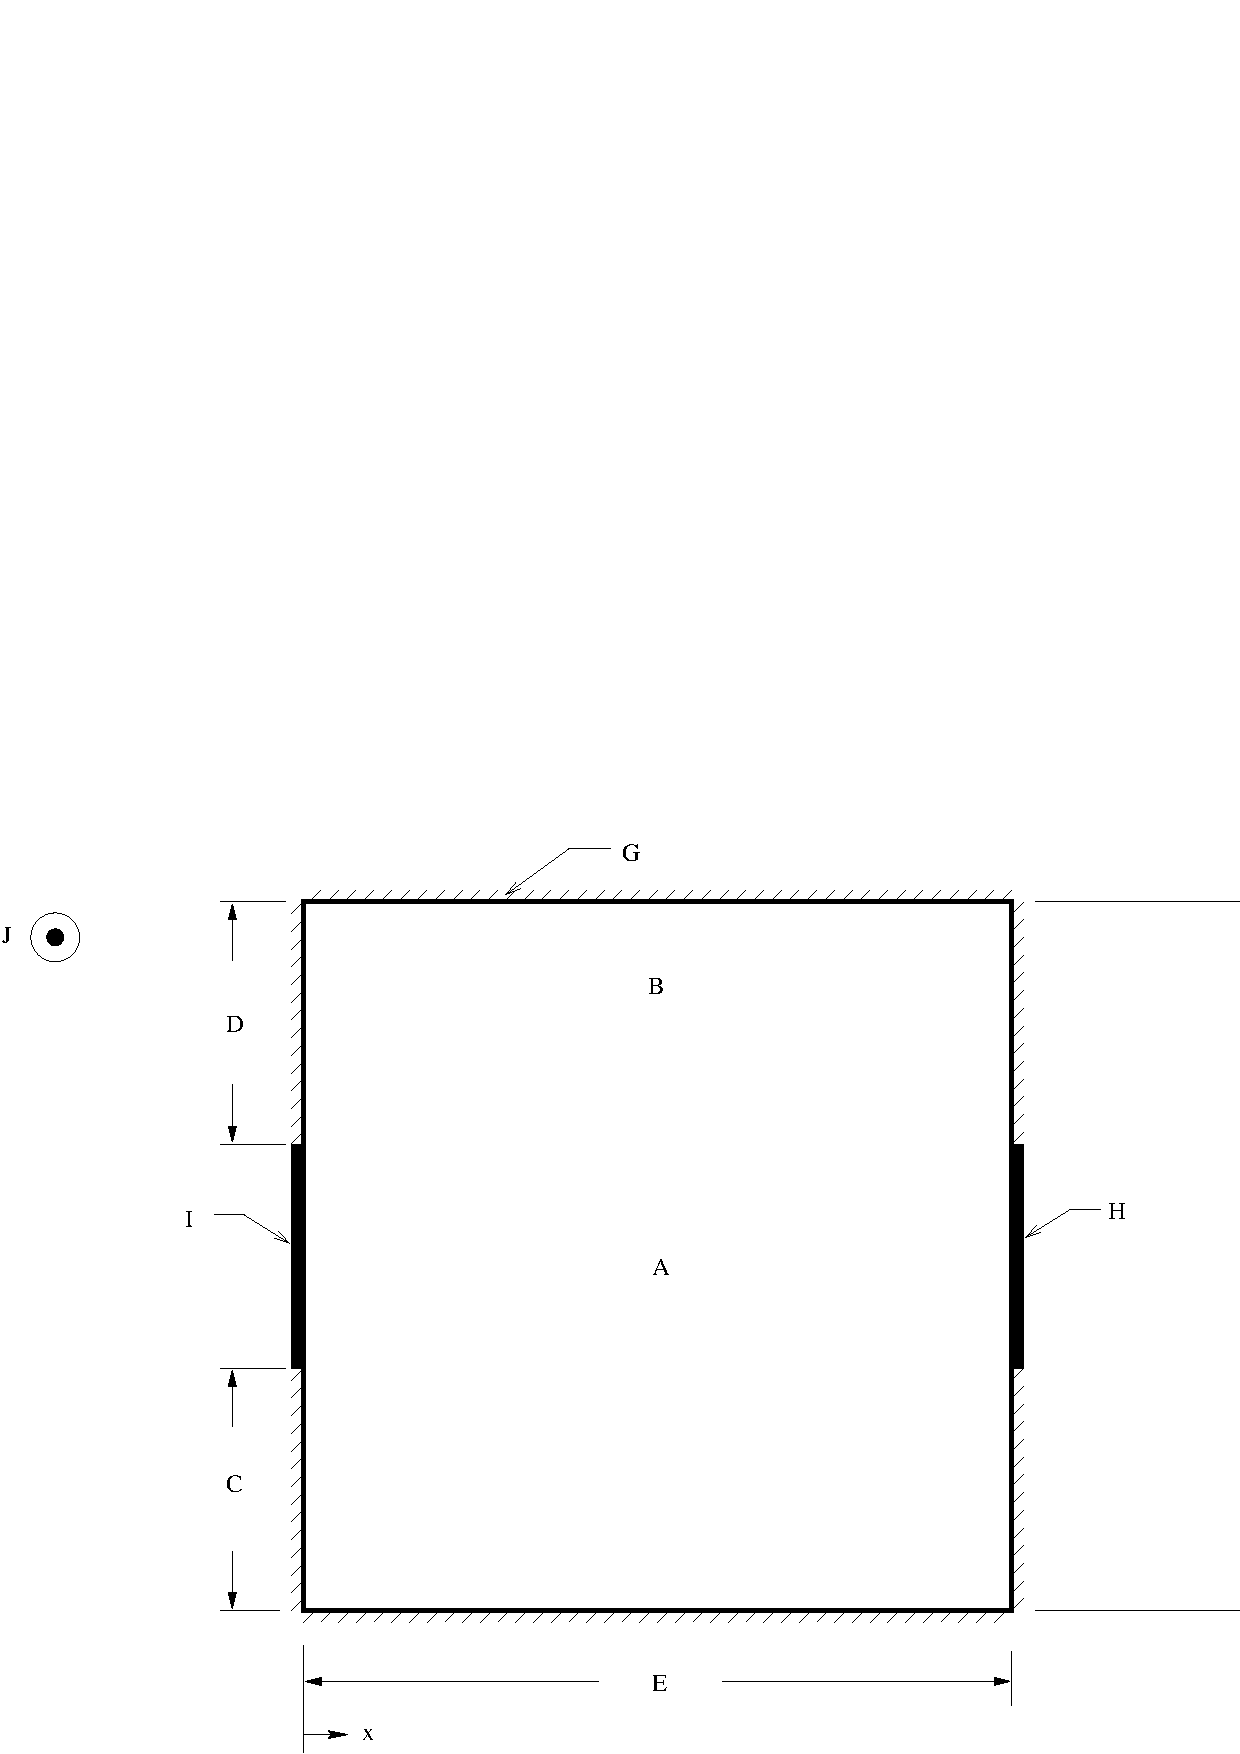
\includegraphics[width=3.5\lengthfigure]{setup_discharge.pdf}
   \caption{Gas discharge test case; all dimensions in millimeters.}
\label{fig:setup_discharge}
\end{figure}
%

The third test case here investigated consists of a gas discharge between two electrodes with a voltage difference of 800 Volts and with the boundary conditions and problem setup schematized in Fig.\ \ref{fig:setup_discharge}. The magnetic field is fixed to 0.8~Tesla and is perpendicular to the computational plane. This results in a significant magnetic field effect on the flow properties due to the electron Hall parameter being of $0.5$. Because such a test case requires a very high number of iterations to converge when using the conventional equations, and because solving a 6-component plasma chemical model requires significantly more computing effort than a 3-component model, it is here decided to reduce the complexity of the chemical model by solving a reduced set of reactions involving only 3 species. The air plasma here considered is thus composed of one type of positive air ions, one type of air neutral molecules, and electrons, with the chemical reactions and mobilities taken from Ref.\ \cite{jcp:2014:parent}. The voltage difference is sufficient for Townsend ionization to occur near the cathode, and the electron-beam power deposited is sufficiently high for a quasi-neutral region to form near the anode. Such a test case is hence well suited to test the performance of the proposed equations in simulating non-neutral cathode sheaths in the presence of a magnetic field typical of plasma magneto-aerodynamics.   




\section{Conclusions}


A new set of equations is here presented to simulate weakly-ionized plasmas in magnetic field using the drift-diffusion fluid model. The proposed set of equations consists of obtaining the potential from the generalized Ohm's law rather than from Gauss's law as is the case in the conventional set of equations. To ensure that Gauss's law is satisfied in non-neutral regions some source terms are added to the ion transport equations. Because the proposed equations are obtained from the same physical model as the conventional equations without introducing new simplifications, they yield the same exact solution either in non-neutral or in quasi-neutral plasma regions (including sheaths near the surfaces as well as regions with significant ambipolar diffusion and drift). 

The present equation set is nonetheless advantaged over the conventional set by not being subject to high stiffness when the plasma includes one or more zones of quasi-neutrality. Reducing the stiffness of the system permits larger integration steplengths to be used which leads to a significant decrease in the number of iterations to reach convergence. Several test cases reveal that the integration steplength can be increased by 20 times or more leading typically to a thirtyfold decrease in  the iteration count whenever a quasi-neutral region of substantial size forms within the plasma. Such gains in convergence acceleration are observed to be independent of the size of the mesh, of the current magnitude, or of the strength of the magnetic and  electric fields.  

Another advantage of the proposed equations is in yielding a higher resolution of the converged solution within (or in the vicinity of) quasi-neutral regions when the externally-applied magnetic field is significant. Indeed, several grid convergence studies of plasmas  with large quasi-neutral regions show that the electric field potential is subject to excessive error when obtained from a potential equation based on Gauss's law. This is attributed to the latter amplifying the error associated with the charged species densities when the net charge tends towards zero. Such an error amplification is avoided when obtaining the potential from the generalized Ohm's law because the latter is not strongly dependent on the net charge density, which leads to the conventional set of equations typically requiring 5 times more nodes to yield the same accuracy as the proposed set within or nearby quasi-neutral regions.    

Not only is the present set of equations advantaged by being less stiff and hence exhibiting faster convergence, but it also results in a more accurate solution on a given mesh. When combined together, these gains in resolution and convergence acceleration result in a one-hundredfold or more increase in computational efficiency for typical steady and unsteady problems involving a quasi-neutral region of substantial size. On the other hand, should the plasma be entirely non-neutral and not include zones  of quasi-neutrality, the proposed equations are observed to converge as rapidly and to exhibit as high a resolution as the conventional set. Because the proposed governing equations yield significant computational advantages with no associated drawback, they are  unconditionally recommended to simulate numerically through the drift-diffusion model weakly-ionized plasmas in the presence of magnetic field.   




\section*{Acknowledgment}

This research was supported by a 2-year Pusan National University Research Grant. 

%% The Appendices part is started with the command \appendix;
%% appendix sections are then done as normal sections
% \appendix



\appendix









\section{Effective Electric Field in Species Reference Frame}
\label{AppendixA}


A justification is here given to why the effective electric field must be determined in the electron reference frame rather than in the neutrals reference frame when computing the electron mobility and the Townsend ionization rates. 

Let us start from the electron energy transport equation as taken from Ref.\ \cite[page 34]{book:1991:raizer}:
%
\begin{equation}
  \frac{\partial }{\partial t} \left( \frac{3}{2} N_{\rm e} k_{\rm B} T_{\rm e} \right)
  + \sum_{i=1}^\nd \frac{\partial }{\partial x_i} \left(\frac{5}{2}  N_{\rm e} k_{\rm B} T_{\rm e} \vec{V}_i^{\rm e} \right)
  - \sum_{i=1}^\nd \frac{\partial }{\partial x_i} \kappa_{\rm e} \frac{\partial T_{\rm e}}{\partial x_i}
  =
   \vec{F}^{\rm e}\cdot \vec{V}^{\rm e}
 - \frac{3}{2} N_{\rm e} k_{\rm B} T_{\rm e} \zeta_{\rm e} \nu_{\rm m} - Q_{\rm ei}  
 \end{equation}
%
where $Q_{\rm ei}$ represents the amount of energy the electrons lose in creating new electrons through Townsend
ionization (that is, the product between the ionization potential and the number of electrons per unit volume per unit time created by electron-impact processes), $\kappa_{\rm e}$ is the thermal diffusivity, $\nu_{\rm m}$ the collision frequency, $\vec{F}^{\rm e}$ is the force per unit volume acting on the electrons due to electromagnetic fields in the electron reference frame, and $\zeta_{\rm e}$ is a term function of the effective electric field which can be determined similarly as in Ref.\ \cite{misc:1995:boeuf}.



Consider the energy transport equation in the ``local approximation'' and neglect the unsteady, convective, and diffusive terms. Then, noting that the collision frequency can be written as follows:
%
\begin{equation}
\nu_{\rm m}=\frac{e}{m_{\rm e}\mu_{\rm e}}
\end{equation}
%
we obtain the following expression for the electron temperature:
%
\begin{equation}
  T_{\rm e}  
=  
 \frac{2 m_{\rm e} \mu_{\rm e}}{3 e N_{\rm e} k_{\rm B} \zeta_{\rm e} }
\left(  \vec{F}^{\rm e}\cdot \vec{V}^{\rm e}
 - Q_{\rm ei}\right)
\label{eqn:appendix:Te}
 \end{equation}
%
where the force per unit volume acting on the electrons in the electron reference frame due to electromagnetic fields  corresponds to:
%
\begin{equation}
\vec{F}^{\rm e} = -eN_{\rm e}\left(\vec{E} + \vec{V}^{\rm e} \times \vec{B}\right)
\label{eqn:appendix:Fe}
\end{equation}
%
and where, in the ``local approximation'',  the electron velocity can be taken from Eq.\ (\ref{eqn:Vvector}) neglecting the pressure gradients:
%
\begin{equation}
  \vec{V}^{\rm e}=\vec{V}^{\rm n} - \mu_{\rm e} \left(\vec{E}+\vec{V}^{\rm e} \times \vec{B}\right)
\label{eqn:appendix:Ve}
\end{equation}
% 
Substitute Eq.\ (\ref{eqn:appendix:Ve}) and Eq.\ (\ref{eqn:appendix:Fe}) in Eq.\ (\ref{eqn:appendix:Te}):
%
\begin{equation}
  T_{\rm e}  
=  
 \frac{2 m_{\rm e} \mu_{\rm e}}{3 e N_{\rm e} k_{\rm B} \zeta_{\rm e} }
\left( -e N_{\rm e} \left(\vec{E} + \vec{V}^{\rm e} \times \vec{B}\right)\cdot \left(\vec{V}^{\rm n} - \mu_{\rm e} \left(\vec{E}+\vec{V}^{\rm e} \times \vec{B}\right)\right)
 - Q_{\rm ei}\right)
 \end{equation}
%
Because the magnitude of the neutrals velocity can be assumed small compared to the magnitude of the electron velocity, the electron temperature becomes:
%
\begin{equation}
  T_{\rm e}  
=  
 \frac{2 m_{\rm e} \mu_{\rm e}}{3 e N_{\rm e} k_{\rm B} \zeta_{\rm e} }
\left(  N_{\rm e} \mu_{\rm e} e |\vec{E}+\vec{V}^{\rm e}\times \vec{B}|^2
 - Q_{\rm ei}\right)
 \end{equation}
%
From the latter, it is clear that in the local approximation the electron temperature is a function of the electric field in the electron reference frame $|\vec{E}+\vec{V}^{\rm e}\times \vec{B}|$, not of the electric field in the laboratory frame $|\vec{E}|$. Because the electron mobility and the Townsend ionization rates depend on the electron temperature, and because the electron temperature is a function of the electric field in the electron reference frame, it follows that the electron mobility and Townsend ionization rates should be determined from an effective electron electric field as follows: 
%
\begin{equation}
 E_{\rm eff}^{\rm e}=|\vec{E}^{\rm e}|=|\vec{E}+\vec{V}^{\rm e}\times\vec{B}| 
\label{eqn:Ee_refframe}
\end{equation}
%
where the electron velocity $\vec{V}^{\rm e}$ can be obtained from Eq.\ (\ref{eqn:V}):
%
\begin{equation}
  \vec{V}^{\rm e}_i = \vec{V}^{\rm n}_i+\sum_{j=1}^\nd s_{\rm e} \wtilde{\mu}^{\rm e}_{ij}  \vec{E}_j^{\rm n}
             - \sum_{j=1}^\nd  \frac{\wtilde{\mu}^{\rm e}_{ij}}{|C_{\rm e}| N_{\rm e}} \frac{\partial P_{\rm e}}{\partial x_j}
\label{eqn:Ve_refframe}
\end{equation}
%
Thus, to find $E_{\rm eff}^{\rm e}$, proceed iteratively: (i) Find $\vec{V}^{\rm e}$ from Eq.\ (\ref{eqn:Ve_refframe}), (ii) Find $E_{\rm eff}^{\rm e}=|\vec{E}^{\rm e}|$ from Eq.\ (\ref{eqn:Ee_refframe}), and (iii) update $\wtilde{\mu}^{\rm e}$ using the latest value of $E_{\rm eff}^{\rm e}$ found in step (ii). Repeat steps (i)-(iii) until $E_{\rm eff}^{\rm e}$ is converged. It is sometimes necessary to under-relax the update of the effective electric field $E_{\rm eff}^{\rm e}$ in the above iterative process in order to prevent some convergence hang, with the relaxation factor typically given a value of 0.9.   

Similarly, it can be demonstrated that the effective electric field  $E_{\rm eff}^k$ needed for the ion mobilities  must also be determined in the reference frame of the charged species under consideration (i.e. $E_{\rm eff}^k=|\vec{E}^k|=|\vec{E}+\vec{V}^k\times \vec{B}|$). The electric field in the ion frame of reference can be obtained for each ion species through the use of Eq.\ (\ref{eqn:V}) by following a similar iterative process as  outlined above. 
 







\bibliographystyle{waflarticle}
\bibliography{all}

\end{document}










